\documentclass{beamer}

\mode<presentation> {

\usetheme{Ilmenau}
\setbeamertemplate{navigation symbols}{}
}

\usepackage{graphicx}
\usepackage{booktabs}
\usepackage[T2A]{fontenc}
\usepackage[utf8]{inputenc}
\usepackage{epigraph}
\usepackage[english,serbian]{babel}

\title[NEAT]{MouseRun}

\author{Nenad Ajvaz, Filip Jovanović, Stefan Kapunac}
\institute[MATF]
{
Univerzitet u Beogradu, Matematički fakultet \\
\medskip
}
\date{24.5.2019.}

\begin{document}

\begin{frame}
\titlepage
\end{frame}

\begin{frame}
\frametitle{Pregled}
\tableofcontents
\end{frame}


\section{Uvod}
\begin{frame} 
\frametitle{Neuro-evolucija}
\begin{itemize}
\item Optimizacija neuronske mreže upotrebom genetskog algoritma
\item \textbf{NEAT} (NeuroEvolution of Augmenting Topologies)
\item Struktura mreže evoluira zajedno sa težinama grana
\item Rezultat - minimalna topologija
\end{itemize}
\end{frame}


\begin{frame} 
\frametitle{Video igra MouseRun}
\begin{columns}[c]
\column{.45\textwidth}
\begin{itemize}
\item Miš beži od mačke
\item Sir mu donosi energiju 
\item Bare ga usporavaju
\item Mišolovke ga ubijaju
\end{itemize}

\column{.45\textwidth}
\begin{figure}
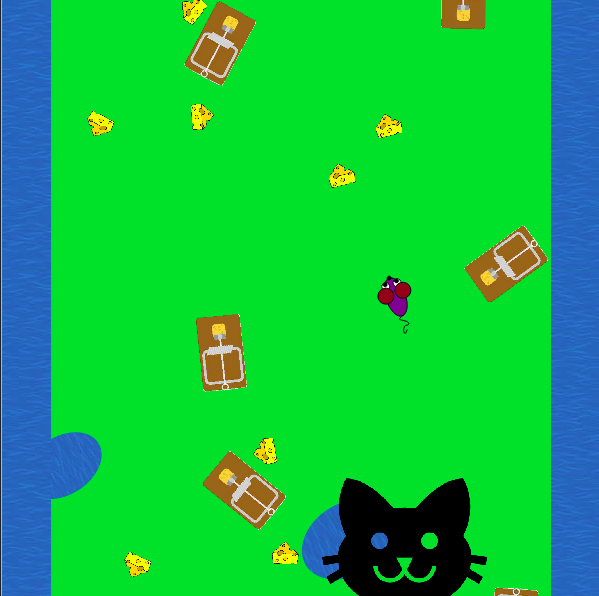
\includegraphics[width=1\linewidth]{images/mouse_run_1.png}
\end{figure}

\end{columns}
\end{frame}

\section{NEAT}
\begin{frame} 
\frametitle{Osnovni koncepti}
\begin{itemize}
\item Indirektno kodiranje mreže
\item Niz grana i čvorova sa globalno jedinstvenim \emph{inovacionim brojevima}
\item Očuvanje raznovrsnosti \emph{specijacijom}
\item Daje vreme novonastalim jedinkama za optimizaciju
\end{itemize}

\begin{figure}
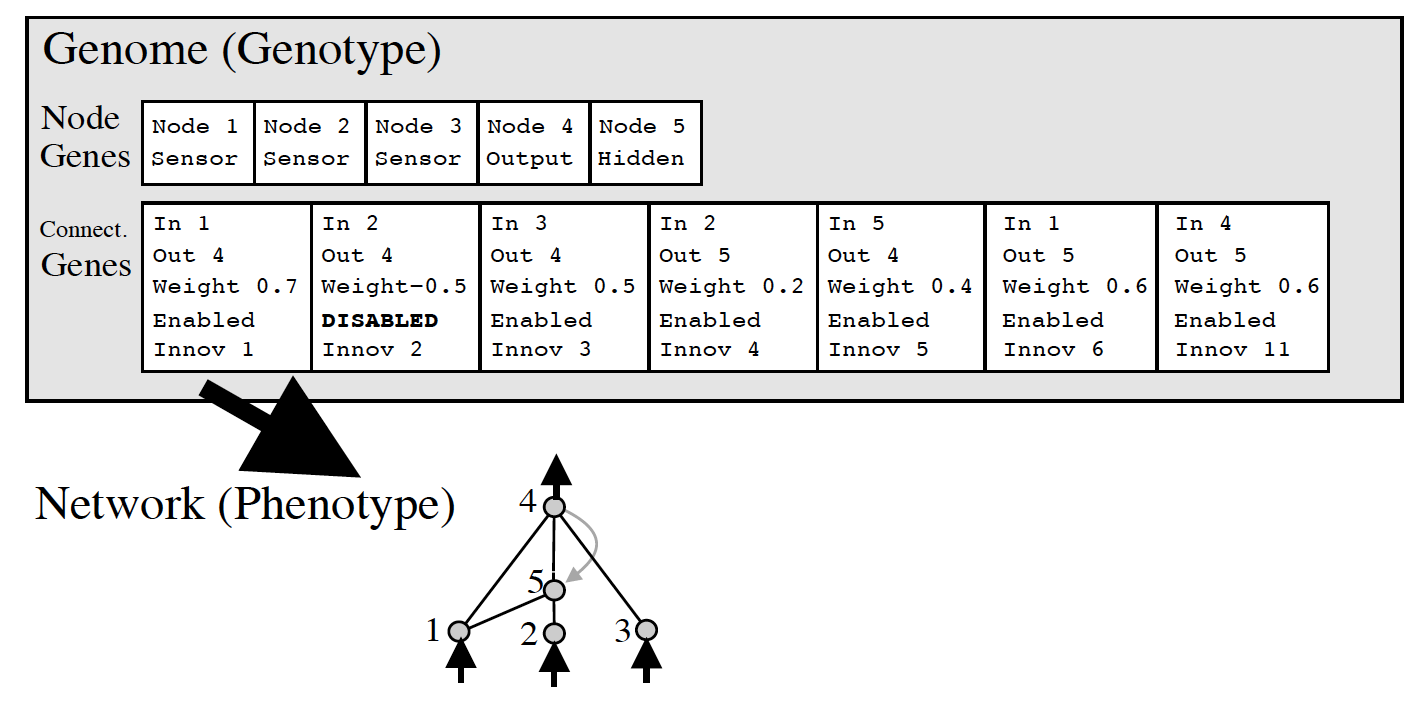
\includegraphics[scale = 0.15]{images/encoding.png}
\end{figure}

\end{frame}

\begin{frame} 
\frametitle{Mutacija}
\begin{columns}[c]
\column{.45\textwidth}
\begin{enumerate}
\item Menjanje težine postojeće grane
\item Dodavanje nove grane
\begin{itemize}
\item Dva nepovezana čvora
\item Jedinstven inovacioni broj grane
\end{itemize}
\item Dodavanje novog čvora
\begin{itemize}
\item Jedna postojeća grana se ,,deli``
\item Jedinstven inovacioni broj čvora
\end{itemize}
\end{enumerate}

\column{.65\textwidth}
\begin{figure}
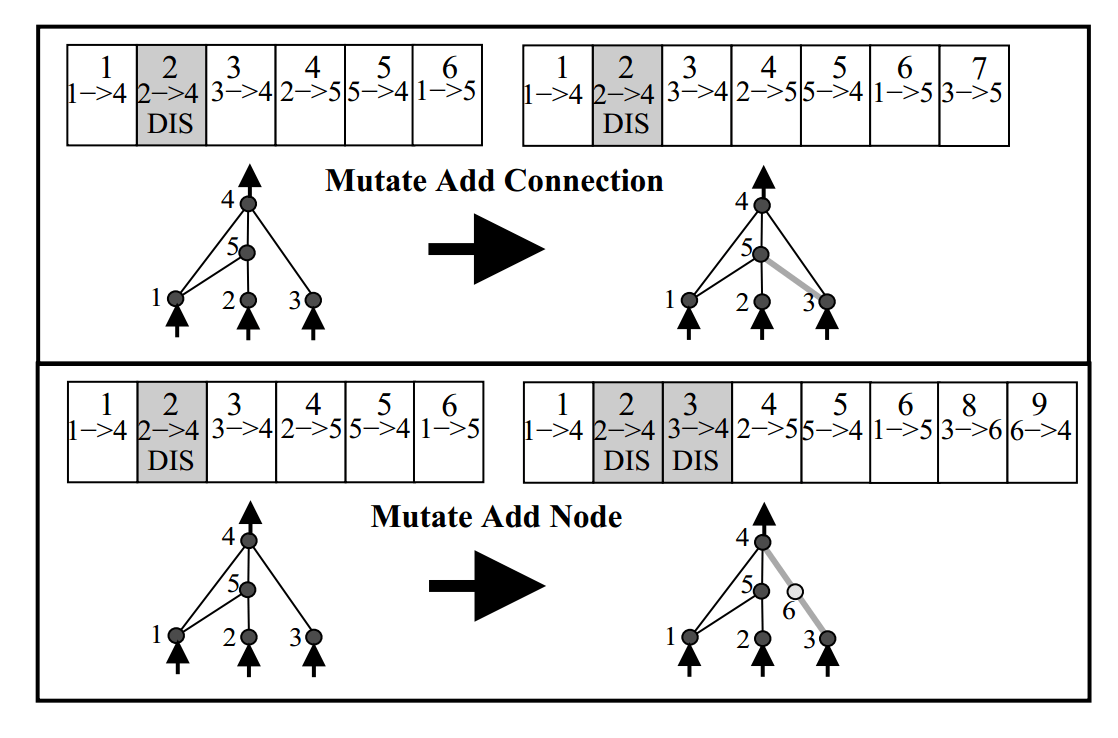
\includegraphics[width=1\linewidth]{images/mutation.png}
\end{figure}
\end{columns}

\end{frame}

\begin{frame} 
\frametitle{Ukrštanje}
\begin{columns}[c]
\column{.45\textwidth}
\begin{itemize}
\item Nema potrebe za analizom topologije
\item Inovacioni brojevi rešavaju problem
\end{itemize}

\column{.65\textwidth}
\begin{figure}
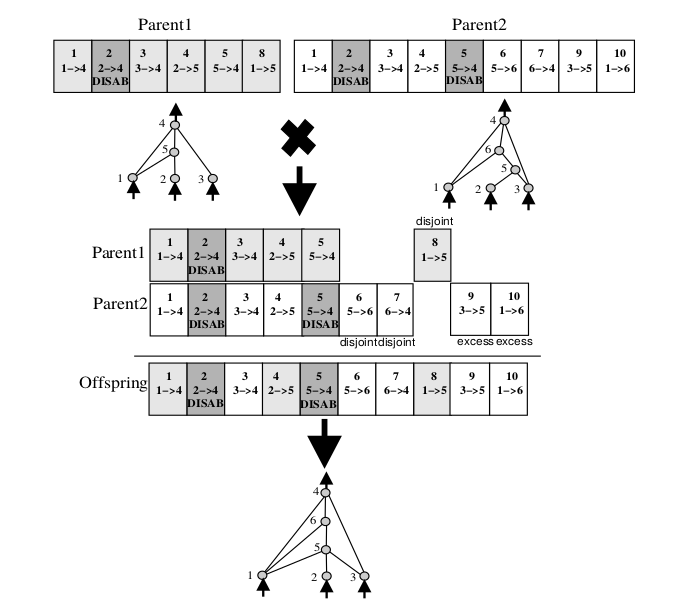
\includegraphics[width=1\linewidth]{images/matching.png}
\end{figure}
\end{columns}
\end{frame}

\section{Implementacija}
\begin{frame} 
\frametitle{Implementacija}
\begin{itemize}
\item C++ i Qt
\item Klase
\begin{itemize}
\item NodeGene
\item ConnectionGene
\item Genome
\item Species
\item Player
\item Game
\item Controller
\item Cheese
\item Cat
\item WaterPool
\end{itemize}
\end{itemize}
\end{frame}

\begin{frame} 
\frametitle{Parametri}
\begin{itemize}
\item Ulazne vrednosti - objekti na sceni u neposrednoj blizini miša (ispred, levo i desno od njega)
\item Izlazne vrednosti - WASD
\item Mutacija:
\begin{itemize}
\item Promena težine: 80\%
\item Nova grana: 5\%
\item Novi čvor: 3\%
\end{itemize}
\item Funkcija aktivacije - modifikovana sigmoidna
\end{itemize}
\end{frame}

\section{Literatura}
\begin{frame}

\nocite{NEAT}
\nocite{ai_techs}

\frametitle{Literatura}
\bibliographystyle{ieeetr}
\bibliography{source}
\end{frame}

\begin{frame}
\frametitle{}
\begin{center}
{\Huge 01001000 01110110 01100001 01101100 01100001 00100001} \\
{\Huge (Hvala!)} \\ 
\bigskip
\bigskip
{\Huge Pitanja?}
\end{center}
\end{frame}



\end{document} 